%Todo
%Table
%Colors
%Check heading structure of tableofcontents and listoffigures etc.




\documentclass[12pt,reqno,oneside]{amsbook}


%%\usepackage[english]{babel}  %Language needs to be specified for accessibility; currently this is not working well with latexml


% Math
\usepackage{amsmath, amssymb, amsthm}

% If you are including computer code the following package is useful.  It is similar to the verbatim package
\usepackage{listings} 

\usepackage{setspace}

%Graphics
\usepackage{graphicx}

% Layout
\usepackage{geometry}
\geometry{margin=1in}

% Theorem environments
\newtheorem{theorem}{Theorem}[chapter]
\newtheorem{lemma}[theorem]{Lemma}
\theoremstyle{definition}
\newtheorem{definition}[theorem]{Definition}

% Hyperref
\usepackage[pdfusetitle]{hyperref}

\begin{document}

% Title metadata.  Make changes here to fit your needs
\newcommand{\thetitle}{A Sample Thesis in Mathematics}

%Edit the following
\newcommand{\institution}{University of Illinois Chicago} 
\newcommand{\degree}{DEGREE}
\newcommand{\programname}{OFFICIAL PROGRAM NAME}
\newcommand{\committee}{Name, Chair, Advisor \\ Name \\ Name\\ Name, Outside Members Need Affiliation Here}
\newcommand{\theauthor}{YOUR NAME AS IT APPEARS ON YOUR EXAM REPORT}
\newcommand{\priordegrees}{BS, University of Wisconsin, 2005\\ Another Prior degree, if Appropriate}
\newcommand{\graduationyear}{YEAR}

% Leave the following for metadata
\author{\theauthor}
\title{\thetitle}
\date{\today}

\frontmatter

% Custom title page
% Take care in making substantial changes to this as it needs to still work with latexml
\begin{titlepage}
    \centering
	{\Large {\textbf{\thetitle}}}  \par}
    \vspace{2cm}
    {BY\par}
    \vspace{0.5cm}
    {\theauthor}\\
    {\priordegrees}\\
    \vspace{2cm}
	THESIS [PhD candidates may use DISSERTATION here instead]\\
	\vspace{1cm}
	Submitted as partial fulfillment of the requirements\\ \vspace{0.2cm}
	for the degree of {\degree} in {\programname} \\ \vspace{0.2cm}
	in the Graudate College of the \\  \vspace{0.2cm}
	University of Illinois Chicago, {\graduationyear}\\
	\vspace{1cm}
	Chicago, Illinois
		
	\raggedright
    \vfill
    Defense Committee: \\
    \committee \\
\end{titlepage}

\setcounter{page}{2} %This is UIC requirement, the title page is (i)

%The following is best practice if distributing both an inacccessible PDF and accessible Epub file.  
\chapter*{Accessibility Statement}
\noindent
An accessible EPUB version of this document is available at [URL] or can be obtained by contacting [contact details].


\chapter*{Dedication}


Lorem ipsum dolor sit amet, consectetur adipiscing elit. Sed non risus. Suspendisse lectus tortor, dignissim sit amet, adipiscing nec, ultricies sed, dolor.

\chapter*{Acknowledgements}

Lorem ipsum dolor sit amet, consectetur adipiscing elit. Sed do eiusmod tempor incididunt ut labore et dolore magna aliqua. Ut enim ad minim veniam, quis nostrud exercitation ullamco laboris nisi ut aliquip ex ea commodo consequat.

\chapter*{Preface}

Duis aute irure dolor in reprehenderit in voluptate velit esse cillum dolore eu fugiat nulla pariatur. Excepteur sint occaecat cupidatat non proident, sunt in culpa qui officia deserunt mollit anim id est laborum.

Curabitur pretium tincidunt lacus. Nulla gravida orci a odio. Nullam varius, turpis et commodo pharetra, est eros bibendum elit, nec luctus magna felis sollicitudin mauris.

Integer in mauris eu nibh euismod gravida. Duis ac tellus et risus vulputate vehicula. Donec lobortis risus a elit. Etiam tempor. Ut ullamcorper, ligula eu tempor congue, eros est euismod turpis, id tincidunt sapien risus a quam.

\tableofcontents
\listoffigures
\listoftables

\chapter*{List of Abbreviations}


\chapter*{Summary}

Cras mollis scelerisque nunc. Nullam arcu. Aliquam consequat. Curabitur augue lorem, dapibus quis, laoreet et, pretium ac, nisi. Aenean magna nisl, mollis quis, molestie eu, feugiat in, orci. In hac habitasse platea dictumst.

Maecenas fermentum consequat mi. Donec fermentum. Pellentesque malesuada nulla a mi. Duis sapien sem, aliquet nec, commodo eget, consequat quis, neque. Aliquam faucibus, elit ut dictum aliquet, felis nisl adipiscing sapien, sed malesuada diam lacus eget erat.

Lorem ipsum dolor sit amet, consectetur adipiscing elit. Vivamus luctus urna sed urna ultricies ac tempor dui sagittis. In condimentum facilisis porta.

Sed nec diam eu diam mattis viverra. Nulla fringilla, orci ac euismod semper, magna diam porttitor mauris, quis sollicitudin sapien justo in libero.

Fusce lacinia quam nisi, euismod ultrices nulla malesuada ut. Curabitur sit amet magna quam. Praesent in libero vel turpis pellentesque egestas sit amet vel nunc.

Morbi lectus risus, iaculis vel, suscipit quis, luctus non, massa. Fusce ac turpis quis ligula lacinia aliquet. Mauris ipsum. Nulla metus metus, ullamcorper vel, tincidunt sed, euismod in, nibh.

Quisque volutpat condimentum velit. Class aptent taciti sociosqu ad litora torquent per conubia nostra, per inceptos himenaeos. Nam nec ante. Sed lacinia, urna non tincidunt mattis, tortor neque adipiscing diam, a cursus ipsum ante quis turpis.

Cras elementum ultrices diam. Maecenas ligula massa, varius a, semper congue, euismod non, mi. Proin porttitor, orci nec nonummy molestie, enim est eleifend mi, non fermentum diam nisl sit amet erat.

Duis semper. Duis arcu massa, scelerisque vitae, consequat in, pretium a, enim. Pellentesque congue. Ut in risus volutpat libero pharetra tempor. Cras vestibulum bibendum augue.

Praesent egestas leo in pede. Praesent blandit odio eu enim. Pellentesque sed dui ut augue blandit sodales. Vestibulum ante ipsum primis in faucibus orci luctus et ultrices posuere cubilia Curae.

Aliquam nibh. Mauris ac mauris sed pede pellentesque fermentum. Maecenas adipiscing ante non diam sodales hendrerit.

Ut velit mauris, egestas sed, gravida nec, ornare ut, mi. Aenean ut orci vel massa suscipit pulvinar. Nulla sollicitudin. Fusce varius, ligula non tempus aliquam, nunc turpis ullamcorper nibh, in tempus sapien eros vitae ligula.

Pellentesque rhoncus nunc et augue. Integer id felis. Curabitur aliquet pellentesque diam. Integer quis metus vitae elit lobortis egestas.

Lorem ipsum dolor sit amet, consectetuer adipiscing elit. Morbi vel erat non mauris convallis vehicula. Nulla et sapien. Integer tortor tellus, aliquam faucibus, convallis id, congue eu, quam.

Mauris ullamcorper felis vitae erat. Proin feugiat, augue non elementum posuere, metus purus iaculis lectus, et tristique ligula justo vitae magna.

Aliquam convallis sollicitudin purus. Praesent aliquam, enim at fermentum mollis, ligula massa adipiscing nisl, ac euismod nibh nisl eu lectus.

Fusce vulputate sem at sapien. Vivamus leo. Aliquam euismod libero eu enim. Nulla nec felis sed leo placerat imperdiet. Aenean suscipit nulla in justo.

Suspendisse cursus rutrum augue. Nulla tincidunt tincidunt mi. Curabitur iaculis, lorem vel rhoncus faucibus, felis magna fermentum augue, et ultricies lacus lorem varius purus.

Sed adipiscing ornare risus. Morbi est est, blandit sit amet, sagittis vel, euismod vel, velit. Pellentesque habitant morbi tristique senectus et netus et malesuada fames ac turpis egestas.

Nullam nonummy metus. Vestibulum volutpat pretium libero. Cras id dui. Aenean ut eros et nisl sagittis vestibulum.

Nulla facilisi. Integer lacinia sollicitudin massa. Cras metus. Sed aliquet risus a tortor. Integer id quam.


%% Text

\mainmatter

\doublespacing %other options are \onehalfspacing or \singlespacing

\chapter{Introduction}
This is the introduction chapter. We cite some classic works \cite{Hartshorne,Mumford}.  

Lorem ipsum dolor sit amet, consectetur adipiscing elit. Morbi tincidunt nisi sed neque volutpat, et imperdiet metus congue. Donec interdum, neque at varius vehicula, elit odio tempus sapien, sed finibus lorem felis nec turpis. Aliquam erat volutpat. Mauris vehicula imperdiet erat, non aliquet magna commodo id.

Sed porttitor urna ac ipsum rhoncus, vel dictum risus commodo. Integer ultrices dui sit amet pulvinar tempor. Phasellus nec tellus eu turpis sodales accumsan. Proin ultr


\begin{theorem}\label{thm1}
This is a theorem
\end{theorem}

We reference Theorem \ref{thm1}.

\href{https://www.uic.edu}{University of Illinois Chicago}.

% JPG, JPEG, PNG will work.  PNG and SVG do not work.
\section{Motivation}


\begin{figure}\label{fig1}
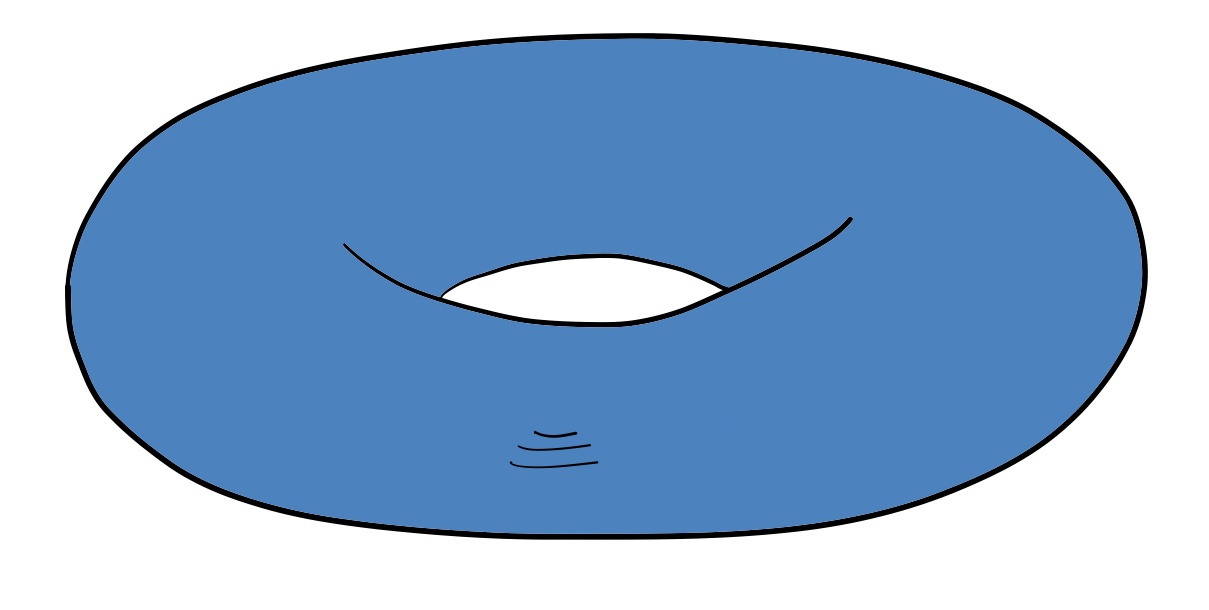
\includegraphics[alt="Description of Image that serves the same purpose",scale=0.3]{torus.jpg}
\caption{This is a torus}
\end{figure}



\begin{figure}\label{fig2}
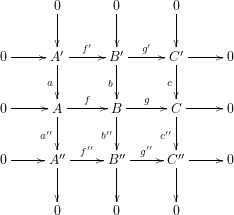
\includegraphics[alt="Description of Image that serves the same purpose",scale=0.8]{figure.png}
\caption{The Snake Lemma}
\end{figure}

%% PDF images do not work
%\begin{figure}\label{fig1}
%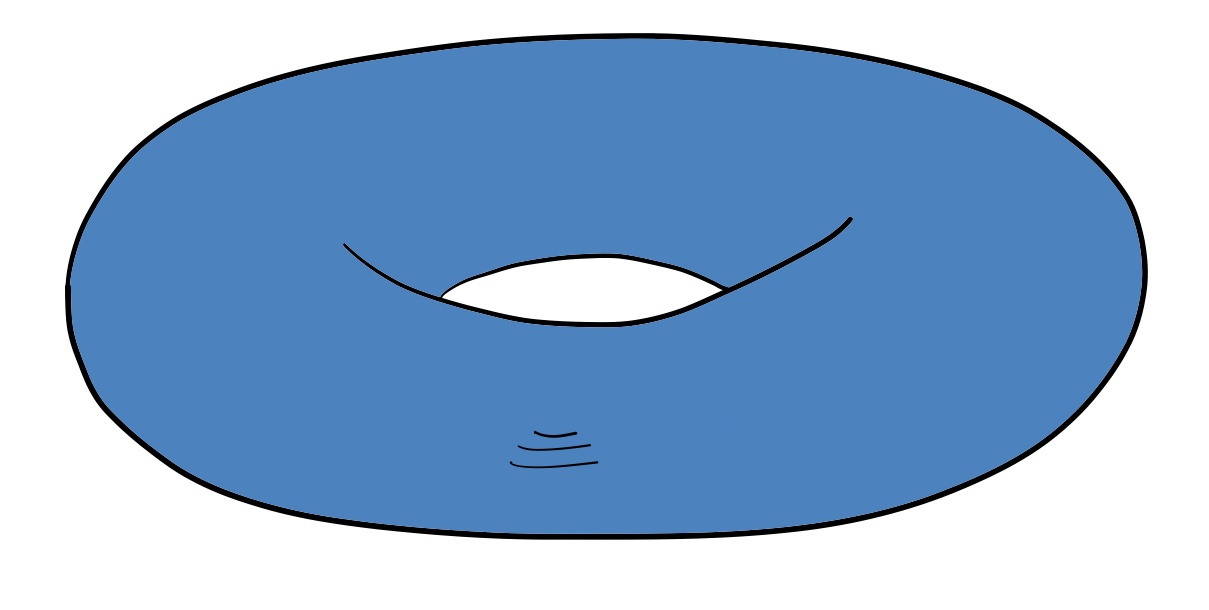
\includegraphics[alt="Description of Image that serves the same purpose",scale=0.3]{torus.pdf}
%\caption{This is a torus pdf}
%\end{figure}

\subsection{Historical context}
A brief overview of how the problem developed.
\begin{equation}\label{eq1}\int_0^1 f(x) dx = 2\end{equation}
How to solve \eqref{eq1}
\subsection{Open questions}
Some questions remain open for future work.

Note: I have not tested the accessibility of this table.
\begin{table}[h]
\centering
\begin{tabular}{cc}
Monkeys & Lions \\
100 & 200
\end{tabular}
\caption{Example Table}
\end{table}


\chapter{Background}
This chapter gives necessary background.

\section{Group theory}
\begin{definition}
A group is a set $G$ with a binary operation satisfying closure, associativity, identity, and inverses.
\end{definition}

\begin{theorem}
Every finite subgroup of the multiplicative group of a field is cyclic.
\end{theorem}

\begin{proof}
This is a standard result from algebra.
\end{proof}

\chapter{Main Results}
Here we present the main contributions of the thesis.

\section{A computer simulation}

% The following works with LaTeXml.  I consider the result accessible, but it might not be 100% WCAG compliant.


\begin{lstlisting}[basicstyle = \singlespacing\ttfamily\small,resetmargins=true,tabsize=5,extendedchars=false]
def factorial(n):
    """Compute the factorial of n recursively."""
    if n == 0:
        return 1
    else:
        return n * factorial(n - 1)

print(f"5! = {factorial(5)}")
\end{lstlisting}



\section{Second main result}
Another significant theorem.

\appendix
\chapter{Technical Lemmas}
Here we collect some supporting lemmas.

\backmatter 
\singlespacing

\begin{thebibliography}{9}


\bibitem{Hartshorne}
R.~Hartshorne, \emph{Algebraic Geometry}, Springer-Verlag, New York, 1977.

\bibitem{Mumford}
D.~Mumford, \emph{Abelian Varieties}, Oxford University Press, 1970.

\bibitem{DraismaEtAl}
J.~Draisma, E.~Horobet, G.~Ottaviani, B.~Sturmfels, and R.~R.~Thomas, 
``The Euclidean distance degree of an algebraic variety,'' 
\emph{arXiv:1309.0049} (2013).  
Available at: \href{https://arxiv.org/abs/1309.0049}{https://arxiv.org/abs/1309.0049}

\end{thebibliography}


\end{document}
